\documentclass[twoside]{article}
\usepackage[utf8]{inputenc}
\usepackage[T1]{fontenc}
\usepackage{xcolor}
\usepackage[utf8]{inputenc}
\usepackage[T1]{fontenc}
\usepackage{xcolor}
\usepackage{amsmath}
\usepackage{tikz}
\usetikzlibrary{fit,positioning}
\usepackage{amssymb}
\usepackage{color}
\usepackage{amsopn,amssymb,thmtools,thm-restate}

\begin{document}

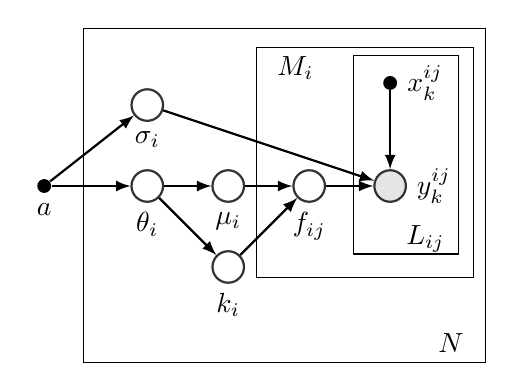
\begin{tikzpicture}
\tikzstyle{main}=[circle, minimum size = 4mm, thick, draw =black!80, node distance = 6mm]
\tikzstyle{para}=[circle, minimum size = 5pt, inner sep=0pt]
\tikzstyle{connect}=[-latex, thick]
\tikzstyle{box}=[rectangle, draw=black!100]
  \node[main, fill = white!100] (theta) [label=below:$\theta_i$] { };
  \node[main] (mu) [right=of theta,label=below:$\mu_i$] {};
  \node[main] (f) [right=of mu,label=below:$f_{ij}$] { };
  \node[main] (k) [below=of mu,label=below:$k_i$] { };
   \node[para, fill = black!100] (alpha) [left=of theta, label=below:$a$] { };
  \node[main, fill = black!10] (y) [right=of f,label=right:$y_{k}^{ij}$] { };
  \node[para, fill = black!100] (x) [above=of y,label=right:$x_{k}^{ij}$] { };
  \node[main, fill = white!100] (sigma) [above=of theta, label=below:$\sigma_i$] { };

  \path (alpha) edge [connect] (theta)
        (alpha) edge [connect] (sigma)
        (sigma) edge [connect] (y)
        (theta) edge [connect] (mu)
        (theta) edge [connect] (k)
		(mu) edge [connect] (f)
		(k) edge [connect] (f)
		(f) edge [connect] (y)
		(x) edge [connect] (y);
  \node[rectangle, inner sep=1mm, fit= (x) (y), label=below right:$L_{ij}$, xshift=-2.4mm, yshift=-6.5mm] {};
  \node[rectangle, inner sep=4.5mm,draw=black!100, fit= (x) (y), xshift=2mm, yshift=-2mm] {};
  \node[rectangle, inner sep=2mm, fit= (x) (y) (f) , label=above left:$M_i$, xshift=6mm, yshift=-3mm] {};
  \node[rectangle, inner sep=6.5mm,draw=black!100, fit= (x) (y) (f) , yshift=-3mm, xshift=2mm] {};
  \node[rectangle, inner sep=0mm, fit= (x) (y) (f) (mu) (k) (sigma) (theta), label=below right:$N$, xshift=7mm, yshift=-5mm] {};
  \node[rectangle, inner sep=8mm,draw=black!100, fit= (x) (y) (f) (mu) (k) (sigma) (theta), yshift=-2mm, xshift=2mm] {};
\end{tikzpicture}

\end{document}